
\chapter{Surgical Method for Analyzing $S(M)$}\label{c4}

The\pageoriginale problem of showing $|S(M)|=1$ breaks into three geometric steps
which we now describe.

\setcounter{step}{0}
\begin{step}\label{c4:step1}
  To show that $[N,f]\in S(M)$ is normally cobordant to $[M,
    id]$. This means that there exists a compact cobordism $W$ and a
  map $F: (W, \partial W)\to (M \times [0, 1], \partial)$ with the
  following properties.
  \begin{enumerate}[(a)]
    \item The boundary $\partial W = N \coprod M$. (Set $N = \partial
      ^+ W, M= \partial^- W$.)
      \item The restriction map $F|_{\partial +w}: \partial^+ W \to M
        \times 1$ is equal to $f$ and $F|_{\partial^-W} : \partial^- W
        \to M \times 0$ is equal to the identity map.
        \item The map $F$ is covered by an isomorphism $\ob{F}: N (W)
          \to \mathcal{E}$ where $N (W)$ is the stable normal bundle of
          $W$ and $\mathcal{E}$ is a bundle over $M \times [0,1]$.
  \end{enumerate}
  From now onwards we will denote a normal cobordism by the triple
  $(W, F, \simeq)$ whre $\simeq$ denotes the isomorphism covering $F$.
\end{step}

\begin{step}\label{c4:step2}
  To show that the cobordism $W$ in Step 1 can be chosen to be an
  $h$-cobordism; i.e., $F$ is actually a homotopy equivalence.
\end{step}

\begin{step}\label{c4:step3}
  To show that the $h$-cobordism $W$ of Step \ref{c4:step2} has
  trivial Whitehead torsion and hence $W$ is a product (Here $\dim M
  \geq 5$.)
\end{step}

We now put an equivalence relation ``$\sim$'' on the set of all normal
cobordisms. We say $(W_1, F_1, \simeq)\sim (W_2, F_2, \simeq _2)$ if
and only if there exists a triple ($\mathcal{W}, \mathcal{F}, \equiv$)
where $\mathcal{W}$ is a cobordism between $W_1$ and $W_2$ and
$\mathcal{F}: \mathcal{W} \to M \times I \times I$ satisfying the
following properties where $I= [0,1]$. The restriction
$\mathcal{F}|_{W_1}: W_1 \to M \times 0 \times I$ is $F_1$, and
$\mathcal{F}|_{W_2} \to M \times 1 \times I$ is $F_2$. Also,
$\mathcal{F}|_{\mathcal{W}-}= id_{M \times I \times 0}$ and
$\mathcal{F}|_{\mathcal{W}^+}$  is a homotopy equivalence, where
$\mathcal{W}^-$ and $\mathcal{W}^+$ are described in Figure 3.

\begin{figure}[H]
  \centering{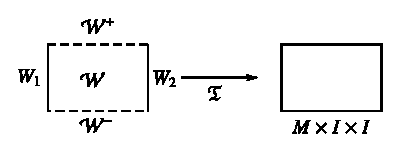
\includegraphics{vol86-figures/fig3.eps}}\\
  Figure 3
\end{figure}

Also,\pageoriginale $\equiv$ is an isomorphism of $\mathcal{N} (\mathcal{W})$ (the
stable normal bundle) to some bundle $\mathcal{E}$ over $M \times I
\times I$ which covers $\mathcal{F}$ and which restricts to $\simeq_1$
and $\simeq_2$ over $W_1$ and $W_2$, respectively. When $m = \dim
M\geq 4$, the equivalence classes of normal cobordisms form a group
which depends only on $\pi_1 (M)$ and the first Stiefel-Whitney class
$w_1 (M) \in H^1 (M, \mathbb{Z}^2)$. When $M$ is orientable, then $w_1
(M) =0$. (We will usually suppress mentioning $w_1 (M)$.) The group of
normal cobordisms modulo equivalence is denoted $L_{m+1} (\pi_1 M)$
where $m= \dim M$. (See \cite{96} for a purely algebraic definition of
the groups $L_n(\pi)$.) The results described above are proven in
\cite{96} and \cite{67}.

\begin{remark*}
  Although the groups $L_n (\pi_1 M)$ are always countable, they are
  sometimes not finitely generated. Cappell \cite{16} for example
  showed that $L_{4n+2} (D_\infty)$ is not finitely generated (for all
  values of $n$) where $D_\infty$ denotes the infinite dihedral
  group. On the other hand, Wall \cite{97} has shown that $L_n
  (\Gamma)$ is finitely generated when $\Gamma$ is a finite group. He
  also here calculated $L_n (\Gamma)$ for $|\Gamma|$ odd. And Wall
  \cite{96} showed that $L_n (\Gamma) = L_{n+4}(\Gamma)$ for every
  $\Gamma$ (not necessarily finite). 
\end{remark*}

\begin{defi}\label{c4:defi4.1}
  A normal cobordism $(W, F, \simeq)$ is called a special normal
  cobordism if $F|_{W^+}$ is a homeomorphism.
\end{defi}

We note that a positive solution to Step \ref{c4:step2} is equivalent
to showing that the normal cobordism of Step \ref{c4:step1} is $\sim$
to a normal cobordism.

We\pageoriginale can define a stronger equivalence relation $\sim_s$
on the set of special normal cobordisms by requiring the restriction
$\mathcal{F}|_{\mathcal{W}^+}$ of the earlier equivalence relation
$\sim$ to be a homeomorphism. This set of special normal cobordisms
modulo the equivalence relation $\sim_s$ is also an abelian group and
it is naturally identified with $[M \times [0, 1], \partial ;
  G/Top]$. Here, $G/Top$ is an $H$-space and $[X, A; G/\ttop]$ denotes
the set of homotopy classes of maps $f: X \to G/\ttop$ such that
the restriction $f|_{A}=1$; i.e., has constant value the homotopy
identity element in $G/\ttop$.

